\chapter{Calibration de la durée d'attractivité} 
\label{chap:attra}

On s'intéresse ici aux résultats produits par le modèle décrit dans la section~\ref{chap:cde}, à la différence que le modèle calibre aussi la durée d'attractivité $d_A$.
On laisse au modèle la possibilité d'avoir une durée d'attractivité $d_A$ comprise entre 3 et 40 jours.

La figure~\ref{fig:da} montre la fréquence des différentes durées d'attractivité obtenues après la calibration du modèle.
Il y a trois durées d'attractivité qui le modèle semble privilégier : 3 jours, 11 jours et 40 jours.
On notera cependant que les durées égales à 3 jours et 40 jours correspondent aux bornes définies pour la calibration.
Une durée d'attractivité égale à 3 jours semble peu réaliste, une durée d'attractivité de 40 jours ne donne pas des dynamiques d'inflorescences significativement différentes avec les dynamiques d'inflorescences vivantes.
On ne s'intéressera donc qu'aux résultats dont la durée d'attractivité est comprise entre 9 et 16 jours.

\begin{figure}[ht]
 \centering
 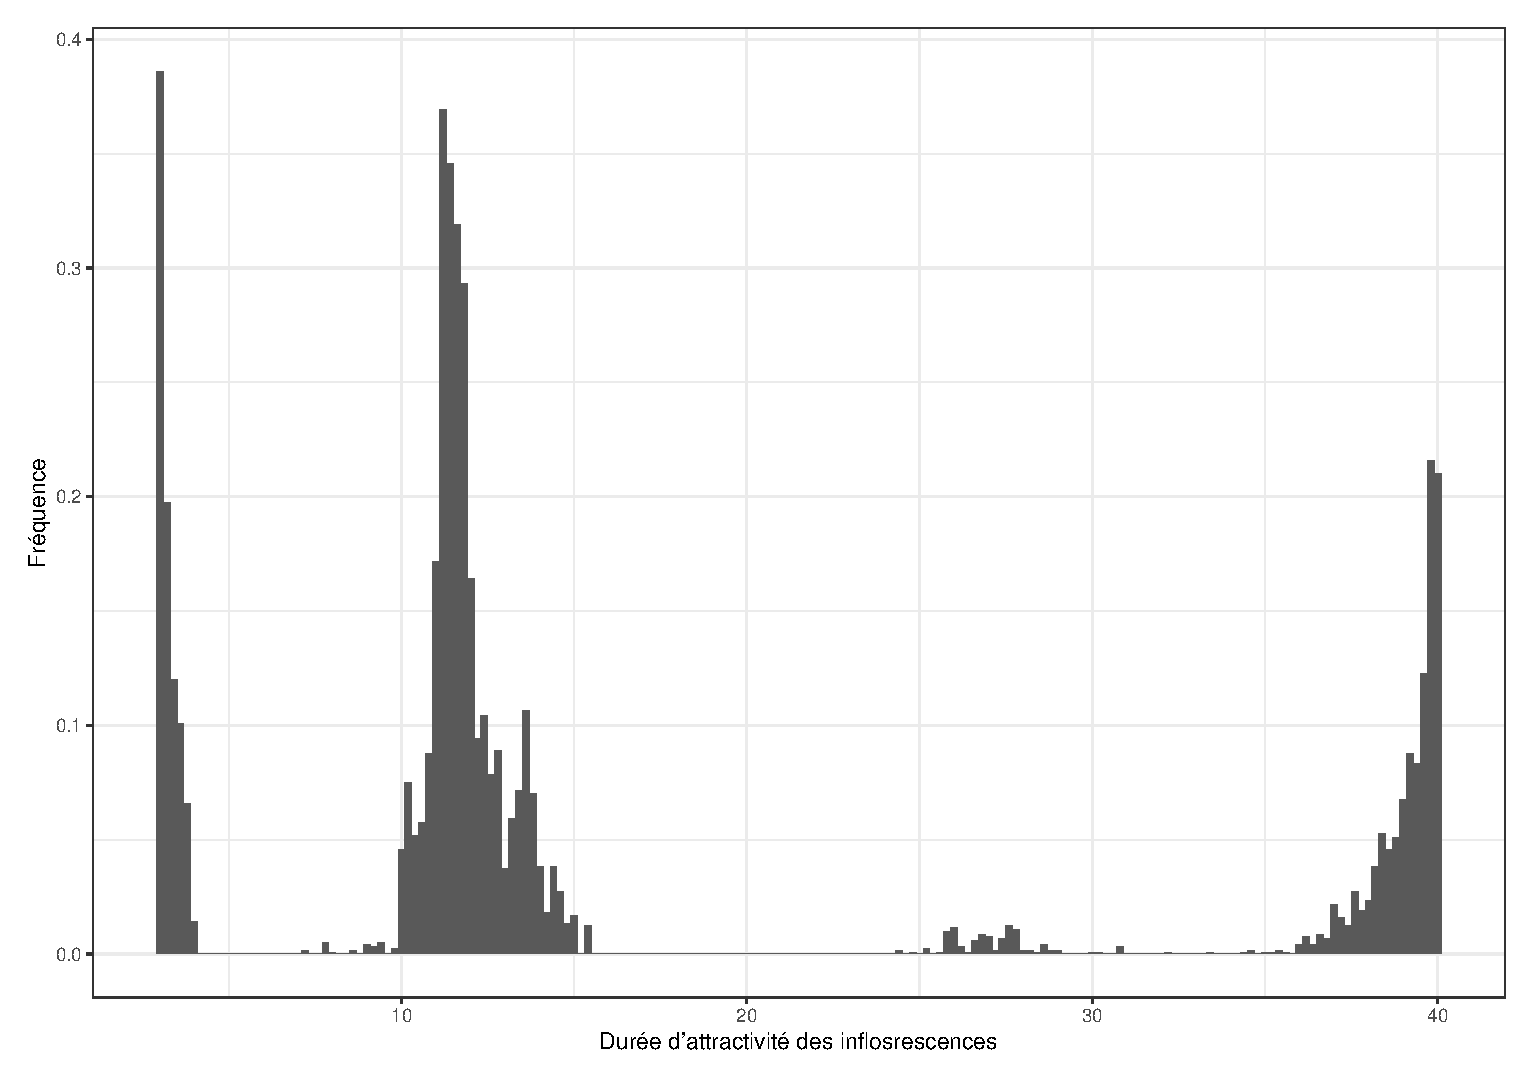
\epsfig{file = plots/dA.eps, scale = 0.43}
 \caption{Fréquence des durées d'attractivité calibrées}
 \label{fig:da}
\end{figure}

Il y a 641 solutions non-dominées dont la durée d'attractivité est comprise entre 9 et 16 jours.
Après classification des solutions, trois solutions types se dégage :
\begin{itemize}
 \item \textbf{Solution--type 1 :} La première solution--type contient beaucoup d'individus exogènes, peu d'échanges entre les trois sous-parcelles, et peu d'individus émergeant de la sous-parcelle EH.
 Il en résulte que, sur les sous-parcelles PS et EH, la population de femelles est essentiellement exogènes. Ce qui paraît peu réaliste.
 En outre, les dynamiques de larves ne sont pas très bien captées.

 Les paramètres associées à cette solution sont :
 \begin{center}
\begin{tabular}{llllllll}
$\gamma$ & $p_{\text{m}}$ & $\mu_{\text{ER}}$ & $\mu_{\text{EH}}$ & $k$ & \texttt{stock} & $E_0\mu_\ell$ & $d_A$\\
0.059 & 0.042 & 0.533 & 0.116 & 1.928 & 500 & 7.517 & 10.3
 \end{tabular}
 \end{center}

 \item \textbf{Solution--type 2 :} Il y a dans la deuxième solution--type des échanges entre les sous-parcelles, cela conduit à des dynamiques de larves assez bien captées sur les sous-parcelles PS et EH.
 En revanche, le niveau d'individus exogènes reste élevé et la dynamique de la sous-parcelle ER toujours aussi mal captée.
 
 Les paramètres produisant cette solution sont :
  \begin{center}
\begin{tabular}{llllllll}
$\gamma$ & $p_{\text{m}}$ & $\mu_{\text{ER}}$ & $\mu_{\text{EH}}$ & $k$ & \texttt{stock} & $E_0\mu_\ell$ & $d_A$\\
0.047 & 0.389 & 0.832 & 0.036 & 1.347 & 522 & 6.466 & 11.5
 \end{tabular}
 \end{center}
 
 \item \textbf{Solution--type 3 :} À la différence des deux autres solutions, il y a peu d'individus exogènes. On note également que les dynamiques de larves captées dans les sous-parcelles PS et EH sont tout à fait satisfaisantes.
 On peut cependant déplorer la mauvaise prédiction sur la sous-parcelle ER.
 
 Les paramètres associées sont :
   \begin{center}
\begin{tabular}{llllllll}
$\gamma$ & $p_{\text{m}}$ & $\mu_{\text{ER}}$ & $\mu_{\text{EH}}$ & $k$ & \texttt{stock} & $E_0\mu_\ell$ & $d_A$\\
0.014 & 0.284 & 0.813 & 0.018 & 0.220 & 6523 & 8.403 & 13.8
 \end{tabular}
 \end{center}
 
\end{itemize}

Les dynamiques sont visibles dans la solution~\ref{fig:C2}.

On notera aussi qu'il n'y a aucune solution avec des individus émergeant de la sous-parcelle EH.


\begin{figure}[ht]
 \centering
 \textbf{Solution--type 1}
 
 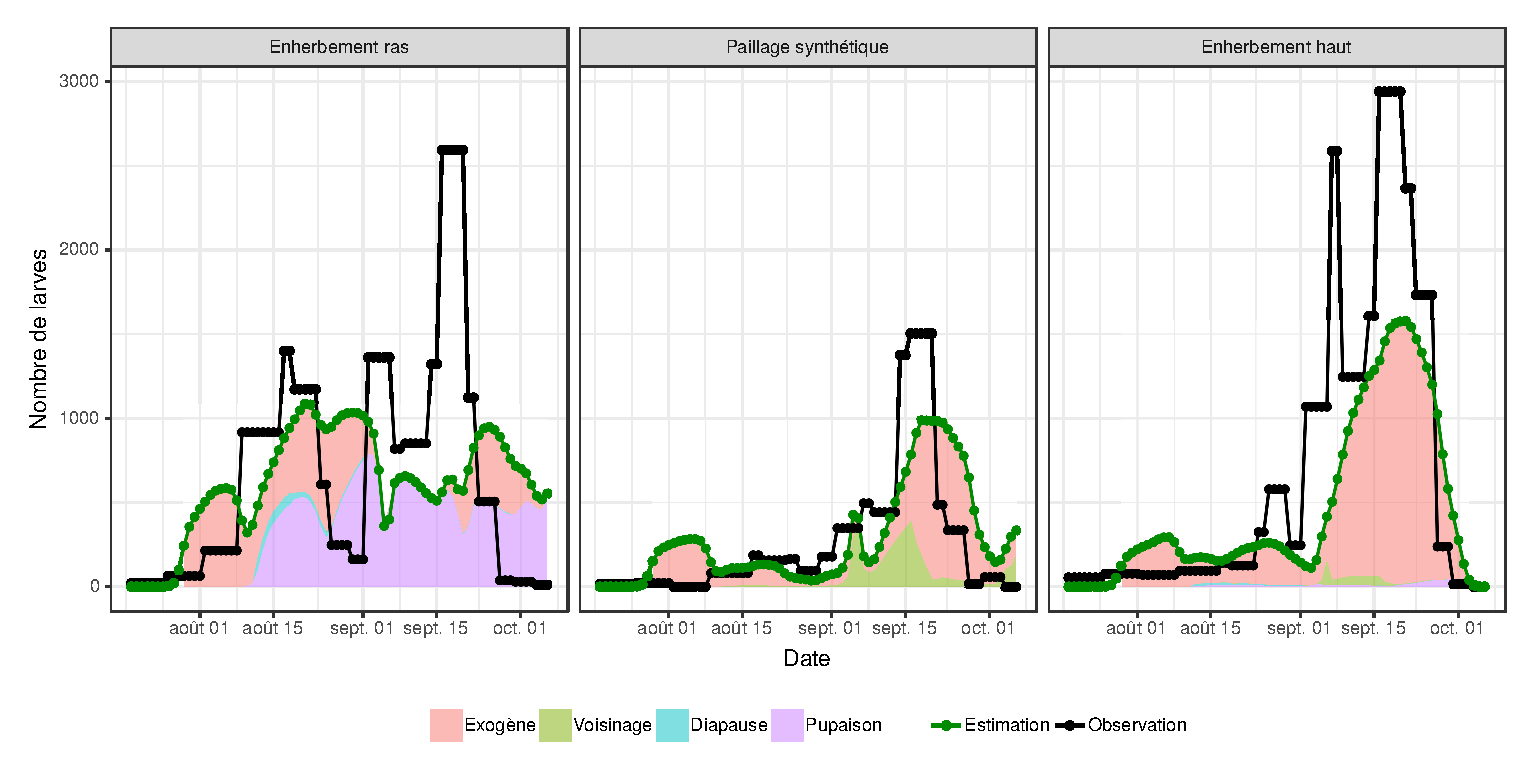
\epsfig{file = plots/C2_1.eps, scale = 0.52}
 
 \textbf{Solution--type 2}
 
 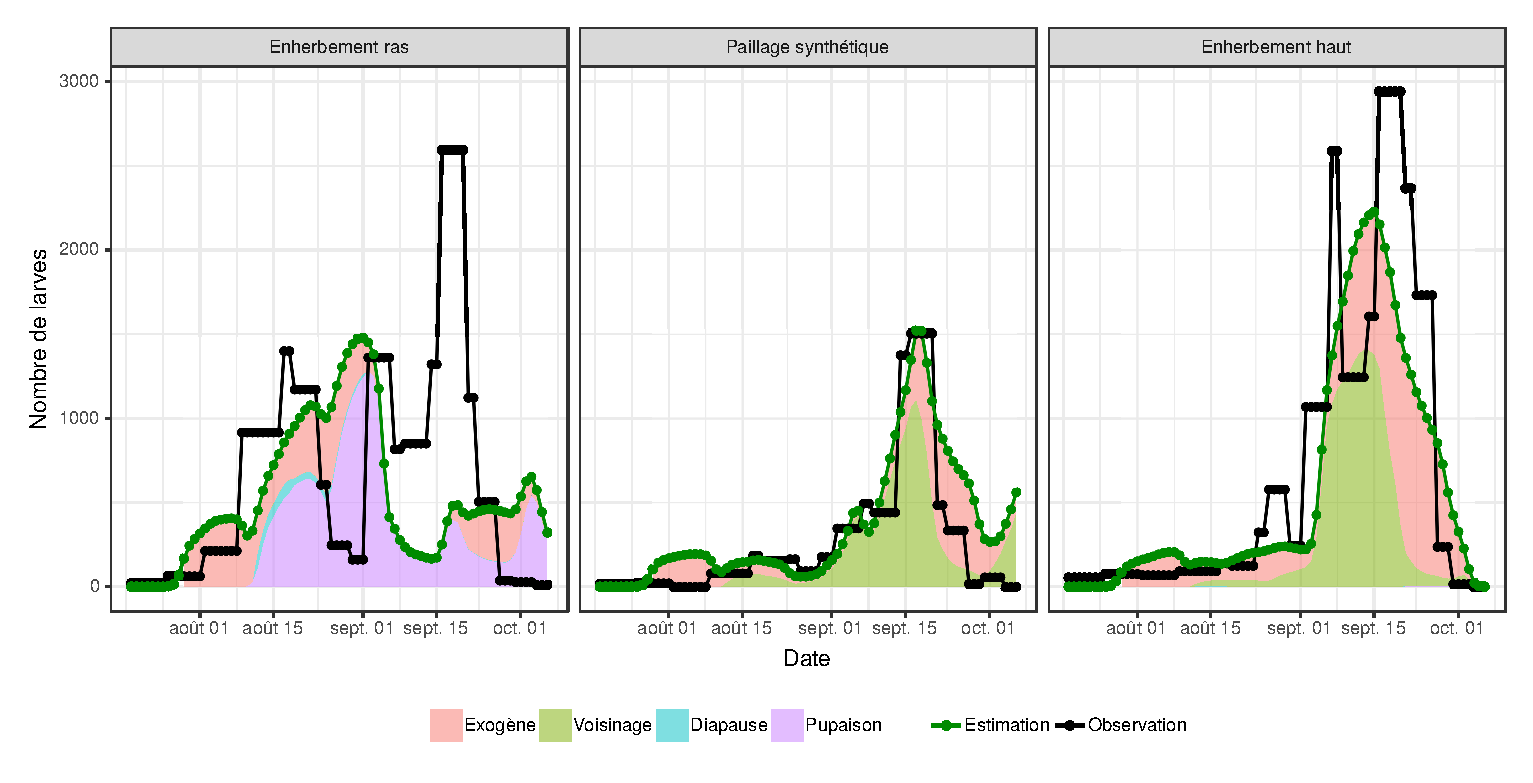
\epsfig{file = plots/C2_2.eps, scale = 0.52}
 
 \textbf{Solution--type 3}
 
 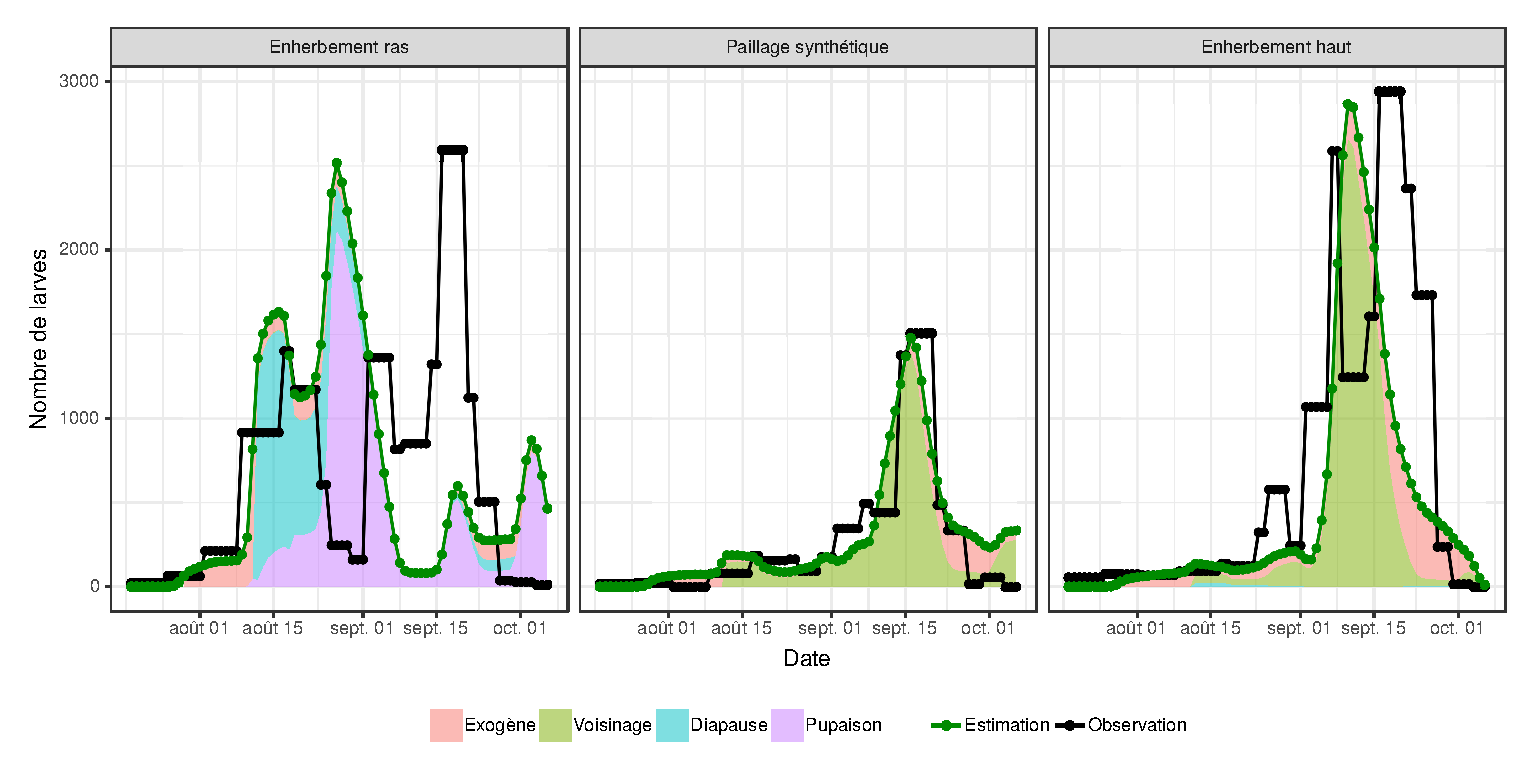
\epsfig{file = plots/C2_3.eps, scale = 0.52}
 \caption{Dynamiques observées et simulées pour chacune des trois solutions--types. La décomposition indiquant la provenance des femelles qui ont pondus les œufs est disponible pour les dynamiques simulées.}
 \label{fig:C2}
\end{figure}
